\documentclass[10pt]{article}

\usepackage{graphicx}
\usepackage{color}
\usepackage[utf8x]{inputenc}
\usepackage[portuges]{babel}
\usepackage{fancyhdr}
\usepackage{nopageno}

\setlength{\textheight}{24.0cm}
\setlength{\textwidth}{17.5cm}
\setlength{\oddsidemargin}{2.0cm}
\setlength{\evensidemargin}{2.0cm}
\setlength{\topmargin}{1.5cm}
\setlength{\headheight}{2cm}
\setlength{\headsep}{1.5cm}
\setlength{\columnsep}{1.5cm}
\addtolength{\oddsidemargin}{-1in}
\addtolength{\evensidemargin}{-1in}
\addtolength{\topmargin}{-1in}
\setlength{\footskip}{0.0cm}
\fancyfoot{}

\pagestyle{fancy}

\lhead{
\includegraphics{udesc.png}}

\begin{document}

\begin{center}
\sc \sc
Universidade do Estado de Santa Catarina \\
Centro de Ciências Tecnológicas \\
Departamento de Ciência da Computação \\
IA - Inteligência Artificial \\
\textbf{Gabriela Salvador Thumé}
\end{center}

\begin{center}
\sc Projeto I
\end{center}


\vspace{10mm}
\textbf{O LABIRINTO DAS ENCHENTES} \\


\vspace{3mm}
Problema do labirinto: encontrar um caminho para um bombeiro ir da posição inicial (1,1) até a posição final (16,16). \\
\vspace{3mm}

O algoritmo que demonstrou melhor desempenho para esse problema foi o A*, por considerar o custo tanto em relação à posição inicial quanto estimando o que faltava até seu objetivo. Mostrou também eficiência em relação aos outros algoritmos por sempre encontrar o melhor caminho e num tempo razoavelmente menor. \\

O algoritmo que encontrou o pior caminho foi o busca cega em profundidade e a busca iterativa tem um custo de tempo muito grande. \\

A seguir são apresentadas as saídas dos algoritmos desenvolvidos para encontrar o caminho do labirinto das enchentes, contando com uma breve explicação sobre cada um e o mapa da saída. \\ 

\vspace{3mm}
\textbf{Busca em Profundidade}
\begin{verbatim}
   Uso: $ ghci
	Prelude> :load labirinto_das_enchentes(busca_profundidade).hs
	*LABIRINTO> inicio

   Saida:
		             BUSCA EM PROFUNDIDADE

	O algoritmo começa num nó raiz e explora tanto quanto possível cada um dos seus ramos, 
antes de retroceder.

[(1,1),  (1,2),  (1,3),  (1,4),  (1,5),  (1,6), (1,7), (1,8),  (1,9), (1,10),
 (1,11), (1,12), (1,13), (1,14), (1,15), (1,16),(2,16),(2,15), (2,14), 
 (2,13), (2,12), (2,11), (2,10), (2,9),  (2,8), (2,7), (2,6),  (2,5), (2,4),
 (2,3),  (2,2),  (2,1),  (3,1),  (4,1),  (5,1), (6,1), (7,1),  (8,1), (8,2), 
 (8,3),  (8,4),  (8,5),  (8,6),  (8,7),  (8,8), (8,9), (8,10), (8,11),(8,12),
 (8,13), (8,14), (8,15), (8,16), (9,16), (9,15),(9,14),(9,13), (9,12), 
 (9,11), (9,10), (9,9),  (9,8),  (9,7),  (9,6), (9,5), (9,4),  (9,3), (9,2),
 (9,1),  (10,1), (10,2), (10,3), (10,4), (10,5),(10,6),(11,6), (11,7),
 (11,8), (11,9), (11,10),(12,10),(12,9), (12,8),(12,7),(12,6), (12,5),
 (12,4), (12,3), (12,2), (12,1), (13,1), (13,2),(13,3),(13,4), (13,5),
 (13,6), (14,6), (14,5), (14,4), (14,3), (14,2),(14,1),(15,1), (15,2),
 (15,3), (15,4), (15,5), (15,6), (15,7), (15,8),(15,9),(15,10),(15,11),
 (15,12),(15,13),(15,14),(15,15),(15,16),(16,16)]

\end{verbatim}

\pagebreak

\begin{verbatim}
X    X    X    X    X    X    X    X    X    X    X    X    X    X    X    X
X    X    X    X    X    X    X    X    X    X    X    X    X    X    X    X
X  |||||               |||||
X  |||||               |||||
X--|||||               |||||--------------------||||||||||||||||||||||||||||||
X  |||||               |||||                    -----
X  |||||||||||||||||||||||||                    -----
X    X    X  --X--  X    X    X    X    X    X  --X--  X    X    X    X    X
X    X    X  --X--  X    X    X    X    X    X  --X--  X    X    X    X    X
X    X    X  --X--  X    X  |||||||||||||||||||||||||
             -----       X    X    X    X    X  |||||-------------------------
X    X    X  --X--  X    X    X    X    X    X  |||||
X    X    X  --X--  X    X                      |||||
X    X    X  --X--  X    X  |||||||||||||||||||||||||
X    X    X  --X--  X    X    X    X    X    X    X    X    X    X    X    X
             -----                                                         X

	Custo total da travessia:159
\end{verbatim}

\vspace{3mm}
\textbf{Busca em largura} \\
\begin{verbatim}
   Uso: $ ghci
	Prelude> :load labirinto_das_enchentes(busca_largura).hs
	*LABIRINTO> inicio

   Saida:
		             BUSCA EM LARGURA

	Faz uma busca em largura, expandindo cada nivel antes de expandir os nós do proximo nível.

[(1,1), (2,1), (3,1), (4,1), (5,1), (6,1), (7,1), (8,1),
 (9,1), (10,1), (11,1), (12,1), (13,1), (14,1), (15,1), (15,2),
 (15,3), (15,4), (15,5), (15,6), (15,7), (15,8), (15,9), (15,10),
 (15,11), (15,12), (15,13), (15,14), (15,15), (15,16), (16,16)]

  X
  X
  X  |||||               |||||
  X  |||||               |||||
--X--|||||               |||||--------------------||||||||||||||||||||||||||||||
  X  |||||               |||||                    -----
  X  |||||||||||||||||||||||||                    -----
  X            -----                              -----
  X            -----                              -----
  X            -----          |||||||||||||||||||||||||
  X            -----                              |||||-------------------------
  X            -----                              |||||
  X            -----                              |||||
  X            -----          |||||||||||||||||||||||||
  X    X    X  --X--  X    X    X    X    X    X    X    X    X    X    X    X
       	       -----                                                         X

\end{verbatim}

\pagebreak

\textbf{Busca com custo uniforme}
\begin{verbatim}
   Uso: $ ghci
	Prelude> :load labirinto_das_enchentes(custo_uniforme).hs
	*LABIRINTO> inicio

   Saida:
		             BUSCA COM CUSTO UNIFORME

	Faz uma busca em largura, porem expande primeiro o no com
menor custo (de acordo com a distancia de manhattan) em relacao a
raiz e garante assim que a primeira solucao encontrada eh a melhor
solucao em relacao a origem. Cuidando que o custo do no seja maior
que do pai.

[(1,1), (2,1), (3,1), (4,1), (5,1), (6,1), (7,1), (8,1), (8,2), (8,3),
 (8,4), (8,5), (9,5), (10,5), (11,5), (12,5), (13,5), (14,5), (15,5),
 (15,6), (15,7), (15,8), (15,9), (15,10), (15,11), (15,12), (15,13),
 (15,14), (15,15), (15,16), (16,16)]


  X
  X
  X  |||||               |||||
  X  |||||               |||||
--X--|||||               |||||--------------------||||||||||||||||||||||||||||||
  X  |||||               |||||                    -----
  X  |||||||||||||||||||||||||                    -----
  X    X    X  --X--  X                           -----
	       -----  X                           -----
	       -----  X       |||||||||||||||||||||||||
	       -----  X                           |||||-------------------------
	       -----  X                           |||||
	       -----  X                           |||||
	       -----  X       |||||||||||||||||||||||||
	       -----  X    X    X    X    X    X    X    X    X    X    X    X
	       -----                                                         X

\end{verbatim}

\pagebreak

\textbf{Busca com aprofundamento iterativo}
\begin{verbatim}
   Uso: $ ghci
	Prelude> :load labirinto_das_enchentes(aprofundamento_iterativo).hs
	*LABIRINTO> inicio

   Saida:
		             BUSCA COM APROFUNDAMENTO ITERATIVO

	A solucao por busca com aprofundamento iterativo eh demorada
pois os nos do nivel inferior d sao geradas uma vez e os filhos da
raiz sao gerados d vezes! (considere o fato de que a primeira solucao
estah na profundidade 30). Nesse problema de caminhos em um
labirinto, temos ciclos, assim cada nó teve de ser identificado com o
numero de sua profundidade tambem, garantindo nao ter estados
repetidos, mas podendo passar por lugares jah antes visitados, porem
por caminhos diferentes.
	Realiza o aprofundamento até um limite i com passos de tamanho n.

	Resultado usando passos de tamanho = 1:


  X    X    X    X    X    X    X    X    X    X
	                                       X
     |||||               |||||                 X
     |||||               |||||                 X
-----|||||               |||||-----------------X--||||||||||||||||||||||||||||||
     |||||               |||||                 X  --X--  X    X    X    X    X
     |||||||||||||||||||||||||                    -----                      X
	       -----                              -----                      X
	       -----                              -----                      X
	       -----          |||||||||||||||||||||||||                      X
	       -----                              |||||----------------------X--
	       -----                              |||||                      X
	       -----                              |||||                      X
	       -----          |||||||||||||||||||||||||                      X
	       -----                                                         X
	       -----                                                         X
\end{verbatim}
\pagebreak
\begin{verbatim}

	Resultado usando passos de tamanho = 5:


  X    X    X    X    X    X    X    X    X    X
	                                       X
     |||||               |||||                 X
     |||||               |||||                 X
-----|||||               |||||-----------------X--||||||||||||||||||||||||||||||
     |||||               |||||                 X  --X--  X    X    X    X    X
     |||||||||||||||||||||||||                    -----                      X
	       -----                              -----                      X
	       -----                              -----                      X
	       -----          |||||||||||||||||||||||||                      X
	       -----                              |||||----------------------X--
	       -----                              |||||                      X
	       -----                              |||||                      X
	       -----          |||||||||||||||||||||||||                      X
	       -----                                                         X
	       -----                                                         X

	Resultado usando passos de tamanho = 10:


  X    X    X    X    X    X    X    X    X    X
	                                       X
     |||||               |||||                 X
     |||||               |||||                 X
-----|||||               |||||-----------------X--||||||||||||||||||||||||||||||
     |||||               |||||                 X  -----  X    X    X    X    X
     |||||||||||||||||||||||||                    -----                      X
	       -----                              -----                      X
	       -----                              -----                      X
	       -----          |||||||||||||||||||||||||                      X
	       -----                              |||||----------------------X--
	       -----                              |||||                      X
	       -----                              |||||                      X
	       -----          |||||||||||||||||||||||||                      X
	       -----                                                         X
	       -----                                                         X

	Os resultados foram iguais porque ele sempre encontra um resultado na profundidade = 30.
A diferença ficou no tempo de execução.
\end{verbatim}

\pagebreak

\textbf{Busca A*}
\begin{verbatim}
   Uso: $ ghci
	Prelude> :load labirinto_das_enchentes(A_estrela).hs
	*LABIRINTO> inicio

   Saida:
		             BUSCA A*

	Faz uma busca em largura, porem expande primeiro o no com menor custo
(de acordo com a distancia de manhattan) em relacao a raiz + em relacao ao 
destino, e garante assim que a primeira solucao encontrada eh a melhor solucao 
em relacao a origem e ao destino. Cuidando que a ordenacao seja pelo maior custo
entre a raiz e o destino entre o no e o seu pai.

	[(1,1), (2,1), (2,2), (2,3), (2,4), (2,5), (2,6), (2,7),
 (3,7), (4,7), (5,7), (6,7), (7,7), (8,7), (9,7), (9,6), (10,6),
 (11,6), (12,6), (13,6), (14,6), (15,6), (16,6), (16,7), (16,8),
 (16,9), (16,10), (16,11), (16,12), (16,13), (16,14), (16,15),
 (16,16)]

  X
  X    X    X    X    X    X    X
     |||||               |||||  X
     |||||               |||||  X
-----|||||               |||||--X-----------------||||||||||||||||||||||||||||||
     |||||               |||||  X                 -----
     |||||||||||||||||||||||||  X                 -----
	       -----            X                 -----
	       -----       X    X                 -----
	       -----       X  |||||||||||||||||||||||||
	       -----       X                      |||||-------------------------
	       -----       X                      |||||
	       -----       X                      |||||
	       -----       X  |||||||||||||||||||||||||
	       -----       X
	       -----       X    X    X    X    X    X    X    X    X    X    X

	Custo total da travessia:37
\end{verbatim}

\pagebreak

\textbf{POSICIONANDO UM MÍNIMO DE OVELHAS NUM CAMPO} \\


\vspace{3mm}
Problema das ovelhas: encontrar um número mínimo de ovelhas num campo com obstáculos, seguindo as regras do cavalo do xadrez, e as configurações possíveis. \\
\vspace{3mm}

Foi utilizada uma busca exaustiva para encontrar o número mínimo de ovelhas suficientes para cobrir todo o campo. Esse número encontrado foi igual a 5.\\

Assim, os algoritmos de otimização posicionaram essas ovelhas no campo de forma a gerar uma configuração aceitável (de forma que nenhuma ovelha ataque a outra e todo o campo esteja coberto). \\

O melhor algoritmo de otimização foi o Simulated Annealing, com uma maior eficiência em tempo. \\

\vspace{20mm}
\centering
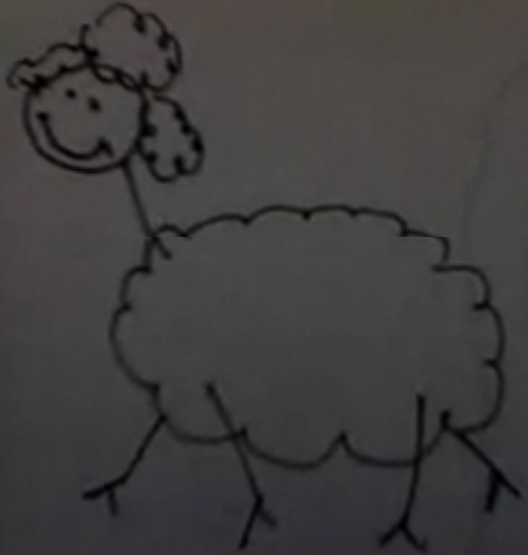
\includegraphics[scale = .5]{ovelha.png}

\pagebreak

\textbf{Busca Exaustiva}
\begin{verbatim}

	Uso:	$ gci
		Prelude> :load ovelhas_no_campo(busca).hs
		*OVELHAS> numero_de_ovelhas

 
        Saída:			     MINIMIZAÇÃO DE OVELHAS

		Partindo de um campo com obstáculos e gramas sem ninguém para cuidar, o algoritmo tenta preencher
com o mínimo de ovelhas possíveis o campo. Começando com uma ovelha, testa todas as configurações 
possíveis e parte para o número de ovelhas mais um.

		Número de ovelhas: 5

\end{verbatim}

\vspace{10mm}
\textbf{Subida de Encosta}
\begin{verbatim}

	Uso:	$ ghci
		Prelude> :load ovelhas_no_campo(subida-a-encosta).hs
		*OVELHAS> otimiza

	Saída:
				     OTIMIZAÇÃO COM HILL CLIMBING

		Procura uma configuração aceitável de 5 ovelhas no tabuleiro. 
Gera uma solução aleatória de início, e a cada nova interação, calcula uma solução vizinha 
(troca um de seus elementos aleatoriamente) e escolhe sempre o de menor custo (calculado por 
quantas ovelhas estão em conflito ou gramas em branco).

		Configuração: [(1,5),(4,3),(1,1),(3,3),(5,3)]

\end{verbatim}

\pagebreak
\textbf{Simulated Annealing}
\begin{verbatim}

	Uso:	$ ghci
		Prelude> :load ovelhas_no_campo(simulated-annealing).hs
		*OVELHAS> otimiza

	Saída:
		*OVELHAS> otimiza
				     OTIMIZAÇÃO COM SIMULATED ANNEALING

		Procura uma configuração aceitável de 5 ovelhas no tabuleiro.
Gera uma solução aleatória de início, e a cada nova interação, calcula uma solução vizinha 
(troca um de seus elementos aleatoriamente) e escolhe o de menor custo (calculado por quantas 
ovelhas estão em conflito ou gramas em branco) OU o de pior custo de acordo com a probabilidade 
obtida por (e^(-maiorCusto-menorCusto)/temperatura).

		Configuração: [(3,4),(3,2),(2,2),(3,5),(3,3)]

\end{verbatim}


\end{document}
